\documentclass[manuscript,review]{acmart}


\usepackage{graphicx}
\usepackage{subcaption}
\usepackage{booktabs}
\usepackage{algorithm}
\usepackage{algpseudocode}
\usepackage{xcolor}
\usepackage{fancyvrb}




\begin{document}

\title{Migrating Code At Scale With LLMs At Google}

\author{Celal Ziftci}
\affiliation{%
  \institution{Google}
  \city{New York}
  \state{NY}
  \country{USA}
}
\email{celal@google.com}

\author{Stoyan Nikolov}
\affiliation{%
  \institution{Google}
  \city{Munich}
  \country{Germany}
}
\email{stoyannk@google.com}

\author{Anna Sj\"ovall}
\affiliation{%
  \institution{Google}
  \city{Munich}
  \country{Germany}
}
\email{annaps@google.com}

\author{Bo Kim}
\affiliation{%
  \institution{Google}
  \city{New York}
  \state{NY}
  \country{USA}
}
\email{bohyungk@google.com}

\author{Daniele Codecasa}
\affiliation{%
  \institution{Google}
  \city{Munich}
  \country{Germany}
}
\email{cdcs@google.com}

\author{Max Kim}
\affiliation{%
  \institution{Google}
  \city{Mountain View}
  \state{CA}
  \country{USA}
}
\email{maxkim@google.com}



\begin{abstract}
Developers often evolve an existing software system by making
internal changes, called \emph{migration}. Moving to a new framework,
changing implementation to improve efficiency, and upgrading a
dependency to its latest version are examples of migrations.

Migration is a common and typically continuous maintenance
task undertaken either manually or through tooling. Certain 
migrations are labor intensive and costly, developers do not find the
required work rewarding, and they may take years to complete.
Hence, automation is preferred for such migrations.

In this paper, we discuss a large-scale, costly and traditionally
manual migration project at Google, propose a novel automated
algorithm that uses change location discovery and a Large Language
Model (LLM) to aid developers conduct the migration, report the
results of a large case study, and discuss lessons learned.

Our case study on 39 distinct migrations undertaken by three developers 
over twelve months shows that a total of 595 code changes
with 93,574 edits have been submitted, where 74.45\% of the code
changes and 69.46\% of the edits were generated by the LLM. The 
developers reported high satisfaction with the automated tooling, and
estimated a 50\% reduction on the total time spent on the migration
compared to earlier manual migrations.

Our results suggest that our automated, LLM-assisted workflow
can serve as a model for similar initiatives.
\end{abstract}

\keywords{Software, Migration, Refactoring, Transformation, Productivity, LLM}

\maketitle

% =====================================================================
\section{Introduction}
% =====================================================================

Software systems are rarely static. Over their lifetime, they are
repeatedly \emph{migrated}: adapted internally so they keep working
correctly as the surrounding technology landscape changes. Typical
examples include moving a codebase to a new framework, upgrading a
library to a newer major version, or changing an underlying data
representation for efficiency or safety reasons. These migrations are
necessary maintenance work, but they tend to be tedious, span huge
codebases, and touch code written by many engineers over many years,
which makes them costly and error-prone when done purely by hand
\cite{hora2015developers, kula2018developers}.

Historically, migrations have been automated with techniques ranging
from regular-expression search-and-replace to purpose-built code
transformation tools to fully custom domain-specific tooling. Each
approach trades off precision, recall, and maintenance cost
differently, and none handles the enormous diversity of coding styles
in a codebase the size of Google's particularly well. The emergence
of Large Language Models (LLMs) capable of reading and generating
code opened up a new possibility: rather than hand-writing exhaustive
transformation rules, an LLM can simply be prompted, in natural
language, to make the required edits itself, while much cheaper
heuristics narrow down \emph{where} in the codebase changes might be
needed.

This paper reports on exactly such a system, built and deployed
inside Google to perform a specific, high-stakes migration: changing
identifier fields in Protocol Buffer schemas from 32-bit integers to
64-bit integers, to avoid identifier space exhaustion as systems grow.
The paper's central contribution is a description of the end-to-end
automated pipeline (reference discovery, automatic categorization,
LLM-driven editing, and multi-stage validation) along with an
evaluation across 39 real migrations carried out by three engineers
over a full year. The study offers a large-scale evaluation of
LLM-assisted code migration in a production environment.

% =====================================================================
\section{Background and Related Work}
% =====================================================================

\subsection{The Migration Problem}
The paper motivates the work with a running example: a proto message
describing a toy in an online store's inventory, where the
\texttt{toy\_id} field is declared as a 32-bit integer. As the number
of toys grows, the store risks exhausting the roughly 2.1 billion
values representable by a signed 32-bit integer, so the field is
widened to a 64-bit integer. This one-line schema edit ripples
outward, though: every place that reads or writes the field, every
bit-manipulation routine that assumed a 32-bit width, and every test
that constructs identifiers with small, in-range sample values needs
to be inspected and, in many cases, changed. Some references are
\emph{direct} (a method call that reads the field), while others are
\emph{indirect}, reached only through data flow, for instance a local
variable later passed into the field setter. The authors note that an
earlier, fully manual version of this same kind of migration took
roughly two years to complete for a single identifier, largely
because regular expressions used to find call sites were
simultaneously too broad (matching unrelated fields with similar
names) and too narrow (missing indirect references and magic numbers
tied to the old bit width).



\subsection{Code Translation and Transformation}
The paper situates its contribution within two long-standing lines of
programming-languages research. \emph{Code translation} concerns
converting code from one language to another, historically via
hand-written parsers and abstract-syntax-tree rewriting rules
\cite{cordy2004txl}, and more recently via learned translation models.
\emph{Code transformation} concerns rewriting code \emph{within} the
same language, traditionally using rule-based languages such as TXL
\cite{cordy2004txl} and Stratego/XT \cite{bravenboer2008stratego}, or
by inferring transformation-by-example rules from a small number of
sample edits. Recent systems such as CodePlan use LLMs with
program-analysis-guided planning to make repository-scale, multi-file
changes \cite{bairi2024codeplan}, and other work automatically mines
reusable transformation rules for library APIs from pull requests
\cite{ramos2023melt}. Closest in spirit are two smaller prior studies:
one evaluating GPT-4 on migrating a handful of methods off an old
version of the SQLAlchemy library \cite{almeida2024library}, and
another studying how developers collaborate with an AI
coding-migration assistant moving a Java 7 codebase to Java 18
\cite{tehrani2024evaluating}. The paper under reproduction differs
from both mainly in scale: it covers 39 distinct migrations, hundreds
of code changes, and tens of thousands of edits, carried out
continuously over a full year inside a production monorepo rather
than as a bounded, small-scale experiment.

\subsection{Automated Refactoring and Rule Mining}
Beyond translation and whole-file transformation, a broader strand of
work targets narrower, well-defined refactoring and transformation
tasks using LLMs paired with static or dynamic program analysis,
mining reusable transformation rules from examples rather than
requiring a developer to hand-write them
\cite{ramos2023melt, bairi2024codeplan}. Compared to this line of
work, the identifier bit-width migration studied in the reproduced
paper is unusual in that a single, uniform intent, widening an
identifier, must be applied consistently across an enormous number of
call sites in several different languages, rather than as a one-off
refactoring of a single method or class.

\subsection{Companion Reports at Google}
The authors note that this paper is a detailed follow-up to two
shorter, earlier write-ups describing the same system: an industry
practice report and an internal engineering blog post, both of which
introduced the system at a higher level before this paper's
twelve-month, 39-identifier case study was available.

The system builds on several pieces of existing Google infrastructure:
a single, monolithic source-code repository shared across the company
\cite{potvin2016google}; Kythe, a code-indexing system used to resolve
symbol references across languages; Critique, Google's internal,
browser-based code review tool \cite{sadowski2018modern}; and an
internally fine-tuned variant of the Gemini family of models
\cite{team2023gemini}, trained using the DIDACT framework for
software-engineering tasks such as code-review comment resolution and
build-error repair.
%=====================================================================
\section{Method}
% =====================================================================

The automated migration system operates as a nightly pipeline with
three main stages, illustrated conceptually in
Figure~\ref{fig:overview}, which repeats until no unresolved
references to a given identifier remain.

\begin{figure}
  \centering
  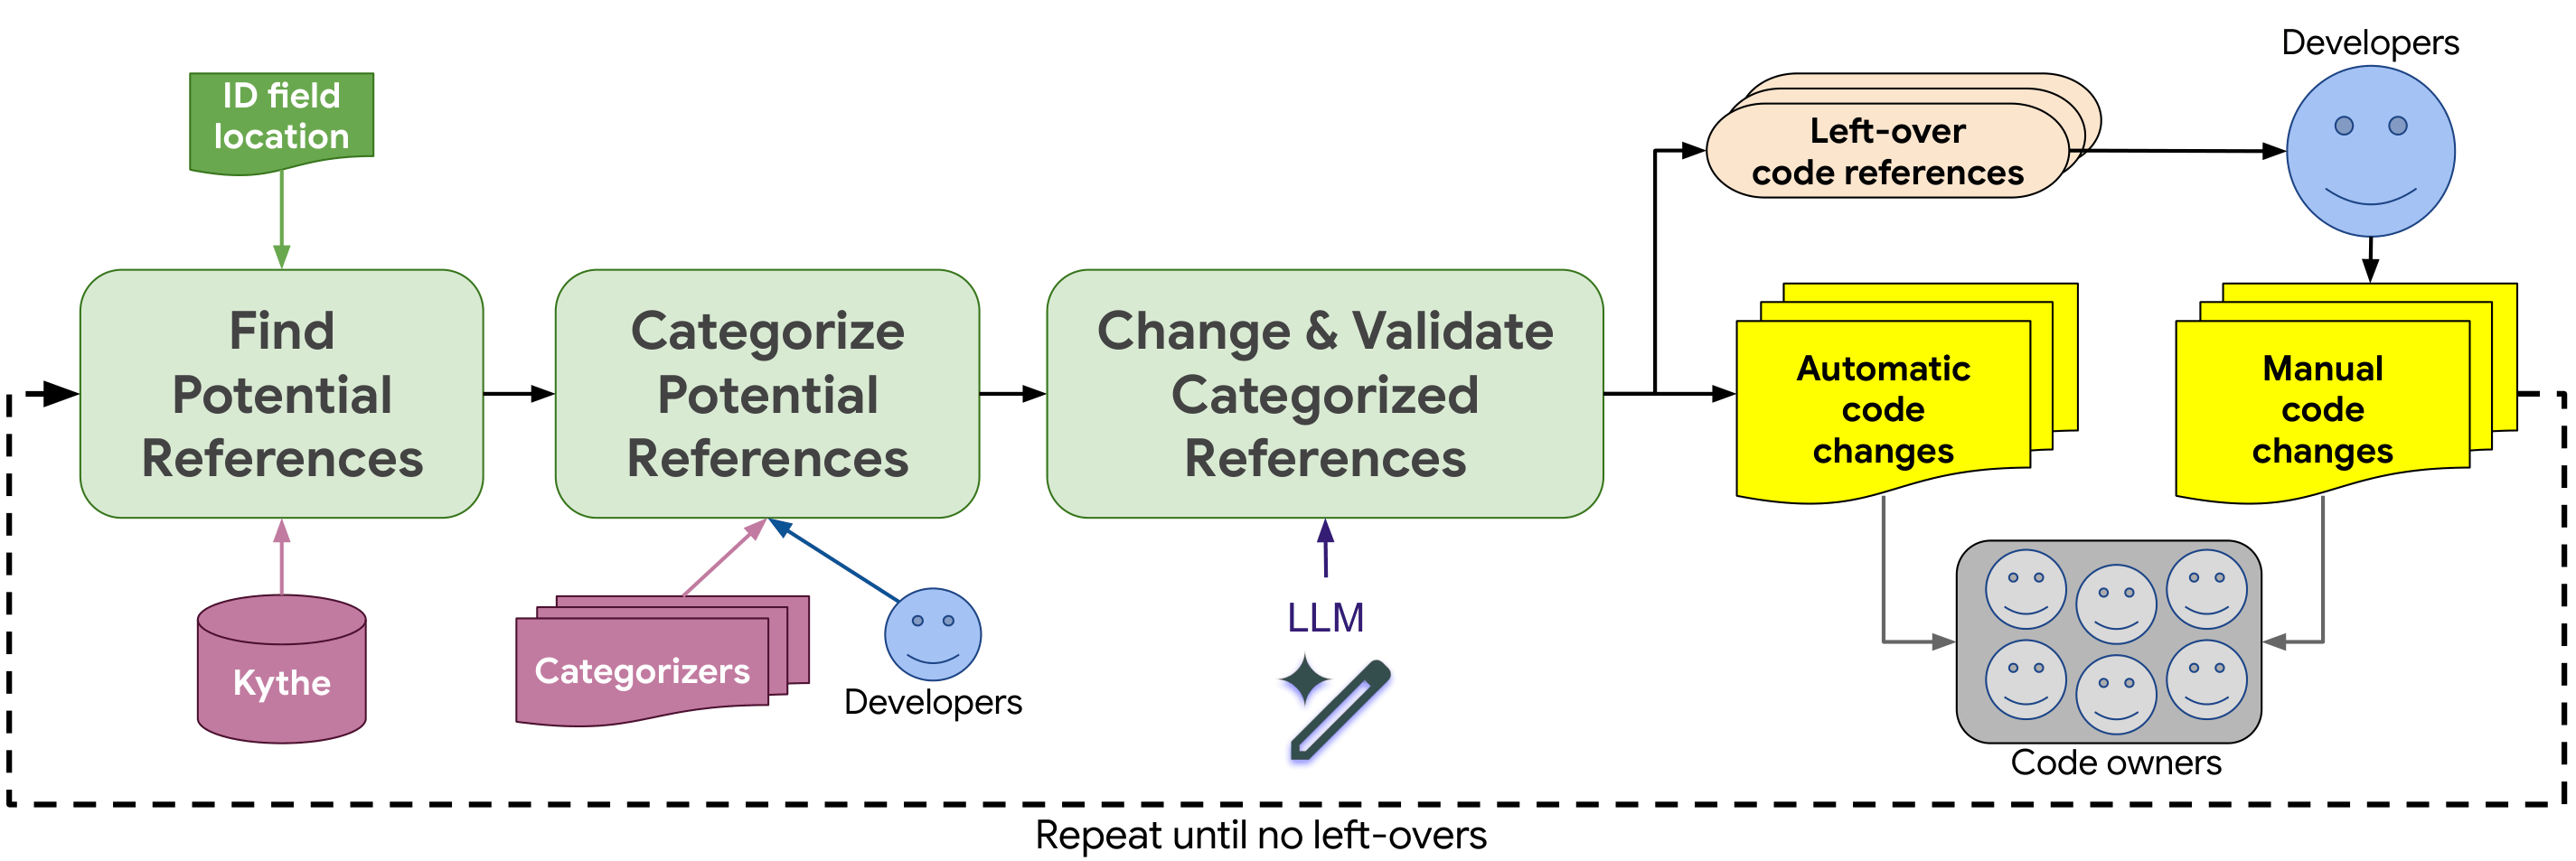
\includegraphics[width=0.8\linewidth]{system-overview.png}
  \caption{High-level overview of the automated migration pipeline
  (screenshot of Figure~1 from the original paper).}
  \label{fig:overview}
\end{figure}

\subsection{Motivating Example Walkthrough}
Before describing each pipeline stage in detail, it helps to ground
all three in a concrete scenario. Suppose a schema field identifying
items in an inventory system is declared as a 32-bit integer, and the
owning team decides to widen it to 64 bits because the item count is
approaching the 32-bit limit. A minimal, adapted illustration of the
kind of code this touches is shown below (this is an original,
simplified stand-in for the style of example used in the paper, not a
reproduction of it):

\begin{Verbatim}[frame=single, framesep=5pt, numbers=left, numbersep=3pt, fontsize=\footnotesize]
int itemId = record.getItemId();
boolean isLegacy = ((itemId >> 31) == 1);

// test code
Record r = Record.newBuilder()
  .setItemId(-7)
  .build();
\end{Verbatim}

Three things happen once the field's declared type changes. First,
the local variable's declared type (\texttt{int}) must widen to match
the field's new accessor return type, or the code will no longer
compile. Second, a bit-shift by 31 that made sense for a 32-bit value
must become a shift by 63 to keep selecting the same high-order bit
on a 64-bit value, a change that a naive text search for the field
name alone would never catch, since the number 31 is not a reference
to the field at all. Third, small hard-coded test values such as
\texttt{-7} technically still compile after the type change but no
longer exercise the new, much larger value range, so tests should
ideally be updated to use identifiers outside the old 32-bit range in
order to catch width-related bugs.

This is exactly the mix of \emph{direct} references (the field
accessor calls), \emph{indirect} references reachable only through
data or control flow (the bit-shift amount), and \emph{semantically
still-valid but no-longer-meaningful} code (the small test literal)
that makes this migration hard to fully automate with text-based
tools alone. It's also what motivates handing the actual editing step
to an LLM that can read and reason about a whole file rather than
matching isolated lines.



\begin{figure}
  \centering
  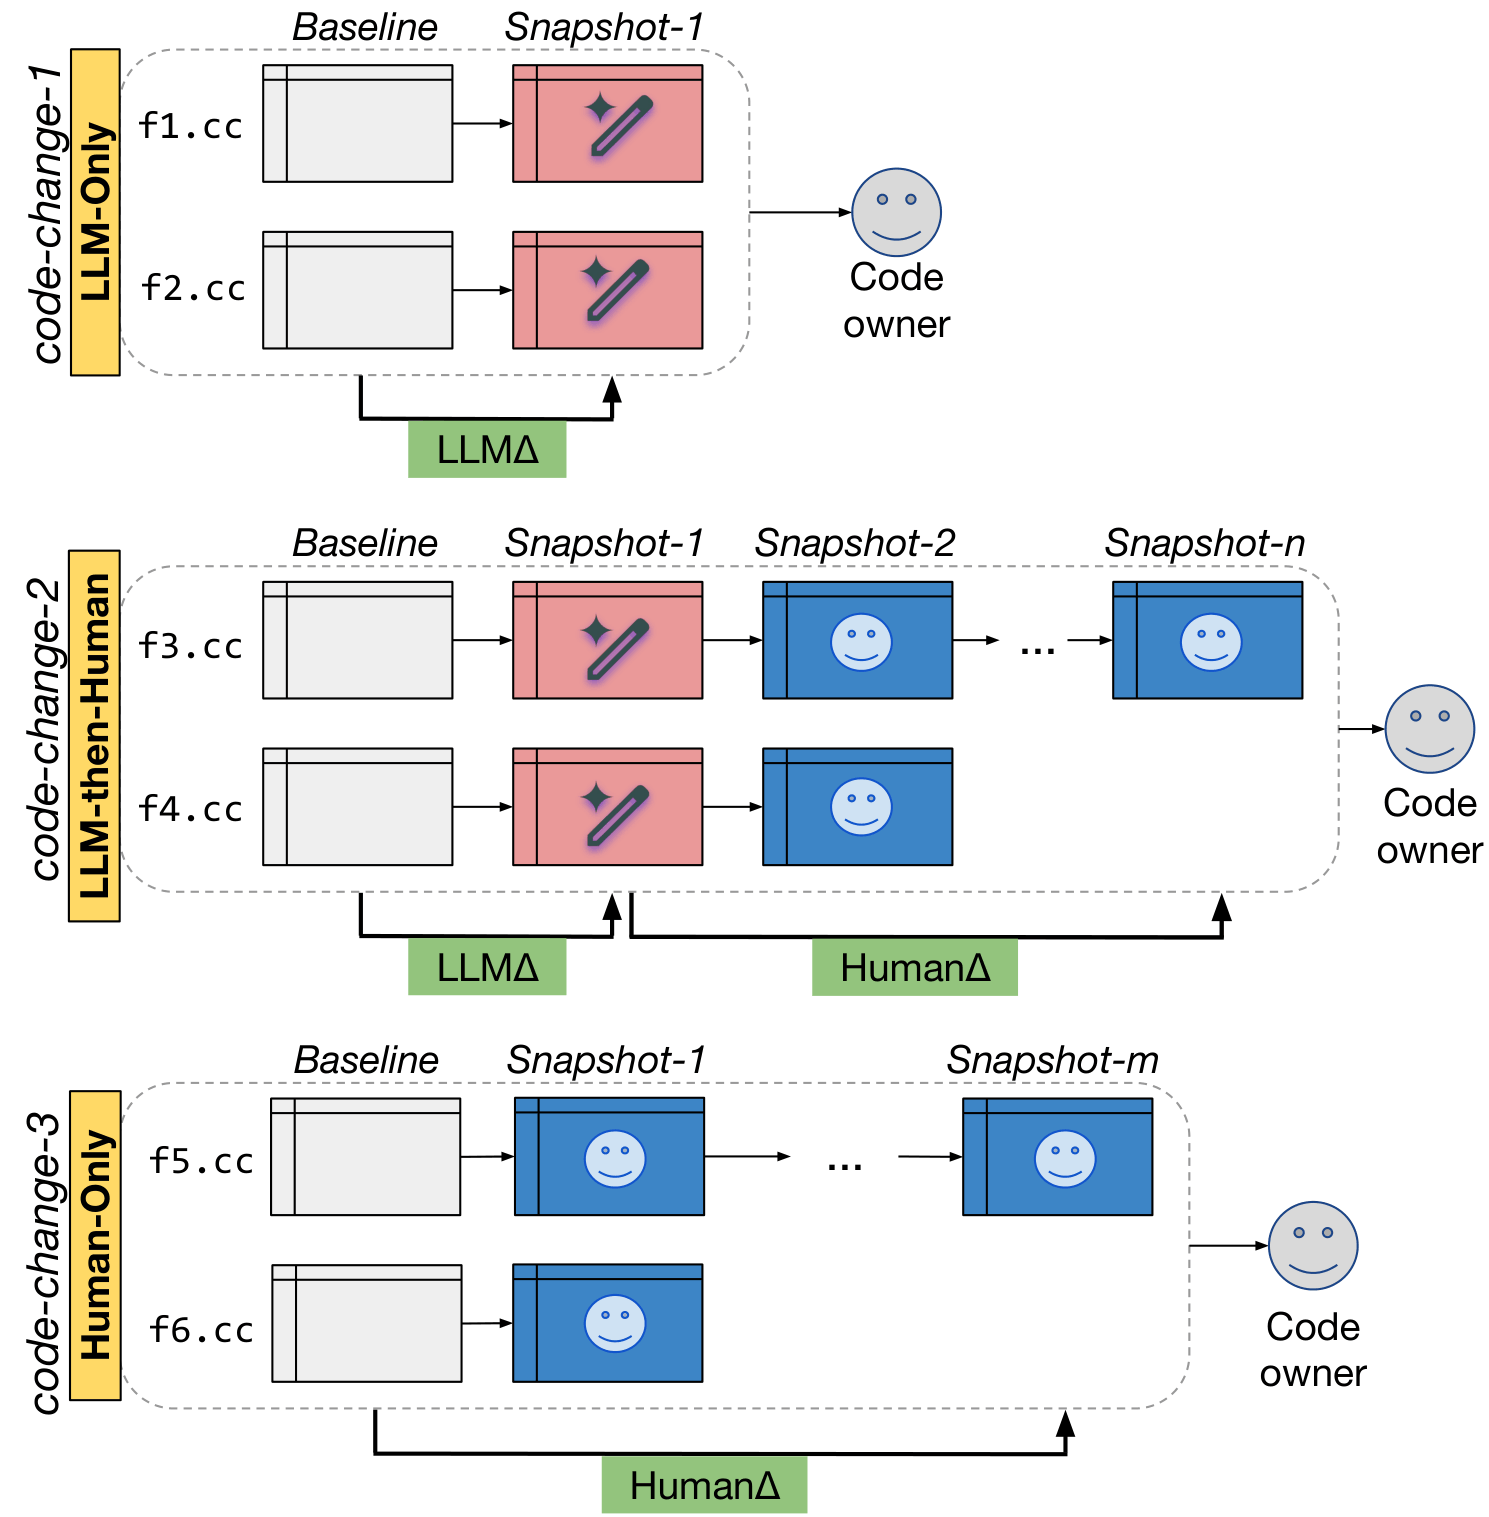
\includegraphics[width=0.8\linewidth]{code-change-types.png}
  \caption{The three code-change categories used to attribute edits
  to the LLM versus to developers (screenshot of Figure~3 from the
  original paper).}
  \label{fig:changetypes}
\end{figure}

Given the location of an identifier field, the system uses Kythe to
find all direct references to it, then recursively expands outward to
indirect references, up to a fixed maximum distance of five hops.
This deliberately produces a superset of the locations that actually
need to change: some flagged locations turn out to be irrelevant
(false positives), and, because the search distance is capped for
practical reasons, some true references beyond five hops may be
missed (false negatives). The authors argue this is an acceptable
trade-off, since more precise techniques such as full data-flow
analysis or AST-based static analysis would be prohibitively expensive
to build and maintain across a codebase written by thousands of
engineers in many languages and styles.

\subsection{Stage 2: Categorizing References}
Each discovered location is run through a bank of lightweight
categorizers, mostly simple regex- and value-range-based heuristics,
that sort it into one of four buckets: \emph{not-migrated} (clearly
still needs updating, high confidence), \emph{irrelevant} (clearly
does not need updating, e.g., a class definition rather than a usage
site), \emph{relevant} (ambiguous, needs closer inspection), or
\emph{left-over} (not confidently classified, queued for manual
developer triage). Developers who investigate left-over locations can
permanently reclassify them via configuration, which the system
consults on subsequent nightly runs.

\subsection{Stage 3: LLM-Driven Change and Validation}
Locations placed in the not-migrated and relevant buckets are handed
to the fine-tuned LLM together with the entire contents of the
containing file and a short natural-language instruction describing
the intended change (e.g., ``update this identifier to a 64-bit type,
and use larger sample values in tests''). The model returns a diff,
applied back onto the original file with a fuzzy diffing algorithm
that tolerates small positional errors in the model's output. Because
model output is non-deterministic even at a fixed temperature, three
independent generation attempts are made per file, and one successful
attempt is chosen at random.

Every LLM-produced change is passed through an ordered chain of
validators, cheapest first, so expensive checks only run on
candidates that already survived the cheap ones. Algorithm~\ref{alg:validation}
summarizes the ordering: a change is discarded (and routed to a human
for manual handling) as soon as it fails any single check.

\begin{algorithm}
\caption{Simplified change-validation pipeline based on Section 3.3 of the original paper.}
\label{alg:validation}
\begin{algorithmic}[1]
\Require candidate file edit produced by the LLM
\If{LLM call did not return successfully}
  \State \Return \textsc{invalid}
\ElsIf{only whitespace/formatting changed}
  \State \Return \textsc{invalid}
\ElsIf{result fails to parse, or AST is unchanged}
  \State \Return \textsc{invalid}
\ElsIf{LLM, when asked, says the change was unnecessary}
  \State \Return \textsc{invalid}
\ElsIf{project fails to build with the change}
  \State \Return \textsc{invalid}
\ElsIf{regression tests fail because of the change}
  \State \Return \textsc{invalid}
\Else
  \State \Return \textsc{ready for review}
\EndIf
\end{algorithmic}
\end{algorithm}

Files that pass every validation step are grouped into code changes
(potentially spanning several files), visually reviewed by the
responsible developer, and sent to the owning team for final approval
and submission through Critique. Figure~\ref{fig:diff} shows, at a
conceptual level, what such a reviewed change looks like inside
Critique's diff view once a file has been edited.


\begin{figure}
  \centering
  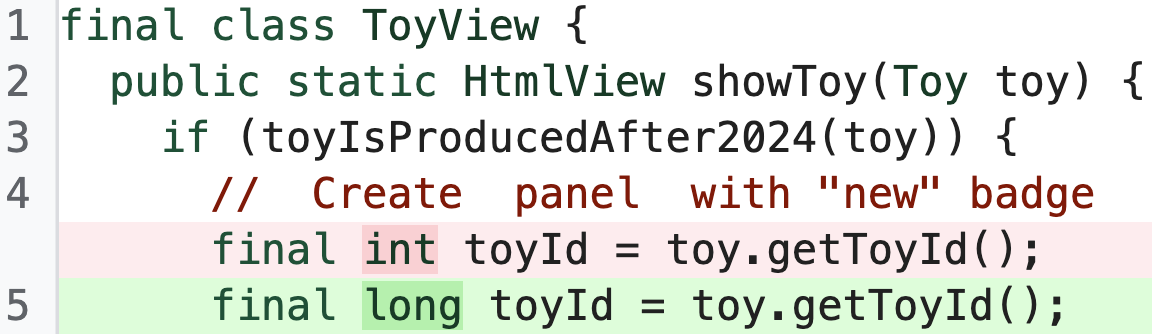
\includegraphics[width=0.75\linewidth]{code-diff.png}
  \caption{Example of a reviewed file edit as it appears in Critique's
  diff view (screenshot of Figure~2 from the original paper).}
  \label{fig:diff}
\end{figure}

\subsection{Prompting Strategy and Observed Edit Patterns}
The natural-language instruction sent to the model alongside a file
is deliberately short and generic rather than file-specific. It
states that the identifier's declared type should change and that
references to it should be updated accordingly, and separately asks
that test code use identifier values large enough to fall outside the
old, narrower range (while keeping the sign of existing negative test
values unchanged). The same wording, translated only insofar as
language-specific accessor-method conventions differ, was reused
across every supported language rather than being hand-tuned per
file.

The authors highlight several qualitative patterns in how the model
responded to this prompt across many files: it reused the same
instruction to correctly update both Java and C++ files despite their
different syntax; it picked the type-appropriate accessor method for
a given language; when a numeric identifier also appeared inside an
embedded SQL query string, it updated both consistently; and, when
given several candidate line numbers containing ambiguous numeric
literals, it could infer which variable was actually the identifier
and edit only that line, rather than blindly changing every suggested
one (Figure~\ref{fig:editexamples}). Developers viewed this
flexibility, handling many languages and edge cases from one generic
instruction, as one of the clearest advantages of an LLM-based
approach over hand-written, per-language transformation rules.


\begin{figure}
  \centering
  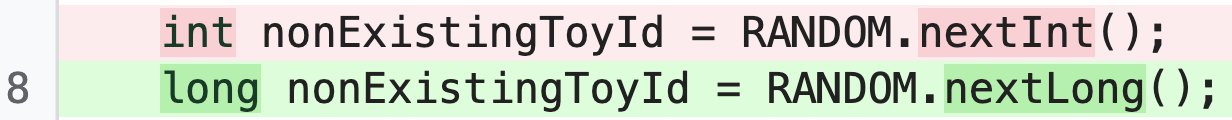
\includegraphics[width=0.7\linewidth]{sample-language-context.png}
  \caption{Examples of qualitative LLM edit behavior observed across
  files and languages (screenshot of Figure~5 from the original
  paper).}
  \label{fig:editexamples}
\end{figure}

\subsection{Evaluation Metrics}
\label{sec:evalmetrics}
To quantify how much of the resulting code was actually written by
the LLM versus by a human, the authors define two metrics based on
Levenshtein edit distance between successive saved snapshots of a
file: \textbf{LLM$\Delta$}, the edit distance between the untouched
baseline and the first LLM-produced snapshot, and
\textbf{Human$\Delta$}, the edit distance between that first snapshot
and the final, human-adjusted snapshot actually submitted. Every
submitted code change is additionally labeled as \emph{LLM-Only}
(entirely from the LLM), \emph{LLM-then-Human} (the LLM produced an
initial version that a developer edited further), or \emph{Human-Only}
(the LLM was not involved at all).

% =====================================================================
\section{Findings and Results}
% =====================================================================

\subsection{Overall Migration Results}
Over twelve months, three developers used the system to migrate 39
distinct identifiers, producing 595 submitted code changes and
93{,}574 individual edits in total. Table~\ref{tab:aggregate}
summarizes the headline numbers reported in the paper.

\begin{table}[t]
\caption{Aggregate statistics reported for the case study (reproduced from Table~1 of the original paper).}
\label{tab:aggregate}
\begin{tabular}{@{}lr@{}}
\toprule
Metric & Value \\
\midrule
Identifiers migrated & 39 \\
Developers involved & 3 \\
Total code changes submitted & 595 \\
\quad LLM-Only & 214 (35.97\%) \\
\quad LLM-then-Human & 229 (38.48\%) \\
\quad Human-Only & 152 (25.55\%) \\
Distinct reviewers & 306 \\
Distinct teams involved & 149 \\
Total edits (all IDs) & 93{,}574 \\
\quad Attributed to the LLM (LLM$\Delta$) & 64{,}996 (69.46\%) \\
\quad Attributed to humans (Human$\Delta$) & 28{,}578 (30.54\%) \\
\bottomrule
\end{tabular}
\end{table}

In other words, 74.45\% of all submitted code changes contained at
least some LLM-authored content (LLM-Only plus LLM-then-Human), and
the LLM was responsible for roughly two-thirds of all edited
characters across the whole study. The size of individual migrations
varied enormously. Some identifiers required edits spread across
hundreds of files in multiple languages, while others were confined
to a single file.

\subsection{Results Across Individual Migrations}
Table~\ref{tab:perid} reproduces the paper's full per-identifier
breakdown, sorted by descending total edit volume (Total$\Delta$).
The two largest migrations, ID-30 and ID-32, together account for a
disproportionate share of all edits in the study, roughly half of the
total across all 39 identifiers combined, while the smallest, such as
ID-10, ID-24, and ID-39, touched only a handful of files. Larger
identifiers also tended to span more programming languages at once:
ID-32 alone touched five different languages, versus a single
language for most of the smaller identifiers.


\begin{table}[t]
\caption{Per-identifier statistics, sorted by descending Total$\Delta$ (reproduced from Table~2 of the original paper).}
\label{tab:perid}
\footnotesize
\begin{tabular}{@{}lrrrr@{}}
\toprule
ID & Total$\Delta$ & \#Changes & \#Files & \#Langs \\
\midrule
ID-30 & 23{,}800 & 39 & 418 & 2 \\
ID-32 & 22{,}822 & 185 & 392 & 5 \\
ID-20 & 16{,}406 & 28 & 175 & 2 \\
ID-28 & 7{,}059 & 29 & 89 & 1 \\
ID-03 & 4{,}594 & 21 & 350 & 4 \\
ID-37 & 2{,}774 & 25 & 58 & 1 \\
ID-06 & 2{,}458 & 23 & 41 & 2 \\
ID-35 & 2{,}039 & 14 & 38 & 2 \\
ID-19 & 1{,}937 & 17 & 21 & 1 \\
ID-18 & 1{,}889 & 20 & 33 & 1 \\
ID-29 & 1{,}825 & 6 & 38 & 1 \\
ID-04 & 1{,}279 & 10 & 27 & 1 \\
ID-31 & 1{,}223 & 15 & 31 & 1 \\
ID-26 & 1{,}151 & 4 & 11 & 1 \\
ID-34 & 1{,}088 & 4 & 16 & 2 \\
ID-09 & 1{,}038 & 6 & 16 & 1 \\
ID-38 & 844 & 8 & 17 & 2 \\
ID-14 & 802 & 7 & 12 & 2 \\
ID-01 & 798 & 16 & 103 & 4 \\
ID-07 & 673 & 7 & 31 & 1 \\
ID-05 & 584 & 5 & 9 & 1 \\
ID-08 & 578 & 6 & 13 & 2 \\
ID-22 & 571 & 2 & 19 & 1 \\
ID-17 & 538 & 4 & 6 & 1 \\
ID-36 & 386 & 5 & 8 & 2 \\
ID-12 & 374 & 5 & 40 & 4 \\
ID-02 & 367 & 10 & 14 & 1 \\
ID-23 & 326 & 10 & 15 & 1 \\
ID-33 & 299 & 7 & 7 & 2 \\
ID-13 & 270 & 8 & 14 & 2 \\
ID-27 & 221 & 5 & 6 & 1 \\
ID-15 & 221 & 11 & 12 & 2 \\
ID-16 & 156 & 9 & 13 & 2 \\
ID-21 & 146 & 3 & 10 & 1 \\
ID-25 & 128 & 7 & 11 & 1 \\
ID-10 & 98 & 1 & 4 & 1 \\
ID-11 & 95 & 7 & 7 & 2 \\
ID-24 & 26 & 2 & 2 & 1 \\
ID-39 & 23 & 1 & 1 & 1 \\
\bottomrule
\end{tabular}
\end{table}


The LLM$\Delta$ share per identifier ranged from close to 100\% for
some identifiers (e.g., ID-10 and ID-39) down to well under half for
others (e.g., ID-15 at 25.34\%). The paper attributes this spread
mainly to two factors discussed further below: how far along
developers were in ramping up on the tool when a given identifier was
tackled, and how much of that identifier's code lived in a language,
such as Dart, that the underlying model handled less well.

\subsection{Developer Experience}
In post-study interviews, the three developers consistently praised
three aspects of the system. First, \emph{end-to-end automation} of
both change discovery and generation gave them a ``continuously
renewed'' migration backlog rather than a one-time, overwhelming task
list. They estimated a roughly 50\% reduction in total time spent
compared with earlier, fully manual migrations, an estimate the
authors note is directionally consistent with the 74.45\% and 69.46\%
automation figures, even though no precise wall-clock timing data was
collected. Second, \emph{automated validation} meant developers no
longer had to manually kick off and babysit build and test runs
before deciding whether a change was ready for review. Third, the
\emph{flexibility of prompting an LLM in natural language} meant the
same simple instruction worked across several languages and coding
idioms, removing the burden of maintaining bespoke transformation
rules for each one.

\subsection{Limitations of the Automated Workflow}
The system was not without limitations, several of which show up
directly in the statistics. \emph{Non-determinism}: because repeated
LLM calls on identical input can produce different diffs, developers
had mixed reactions, sometimes pleased that a retry eventually
succeeded, sometimes frustrated by not knowing how many retries would
be needed before falling back to manual edits. \emph{Context-window
limits}: very large files sometimes could not be passed to the model
in their entirety, causing automatic edits to fail outright.
\emph{Hallucination}: the model sometimes only reformatted a file,
only added a comment next to an already-correct value, or made
unrelated edits, none of which counted as a genuine fix. Hallucinated outputs
 included formatting-only changes, unnecessary comments, and unrelated edits. 
 However, the Human-Only and Human$\Delta$ proportions should not be interpreted as 
 hallucination rates, since manual work also resulted from context 
 limitations, uneven language support, validation failures, and other 
 workflow constraints. \emph{Uneven language support}: the model
handled Java, C++, and Python well but had comparatively weak Dart
support, so identifiers with heavy Dart usage ended up with lower
LLM$\Delta$ shares. \emph{Ramp-up effects}: early in the study,
developers were still learning the tool and tackled small, localized
identifiers largely by hand; as they gained experience they moved on
to larger, more automation-heavy migrations, which the authors say
explains much of the variance seen across individual identifiers.

\subsection{Pre-Existing Failures and Production Rollouts}
Two further sources of friction were largely outside the automated
pipeline's control. First, every code change at Google is expected to
pass the relevant regression test suite before submission; if that
suite already had unrelated, pre-existing failures, the migration's
own validation step would also report a failure even when the LLM's
edit was correct, and developers had to separately track down the
code owners to fix the unrelated failure first. Second, some tests
store their expected output as a serialized ``golden'' file,
regenerated by a specialized tool whenever the code under test
changes. Because the automated pipeline had no way to invoke these
golden-regeneration tools, any test relying on stored goldens would
fail the pipeline's test-validation step regardless of whether the
underlying code change was correct, again pushing that file into the
manual, Human-Only bucket.

Most of the 39 identifiers were small and localized enough that, once
submitted, no further coordination was needed. The two largest and
most widely used identifiers, ID-30 and ID-32, were the exception:
because their blast radius potentially touched many downstream teams,
the resulting changes were rolled out to production gradually, with
affected teams watching for regressions, rather than shipped all at
once. The automated pipeline offered no direct support for this
staged-rollout process; it remained a manual, judgment-driven step
carried out by the developers and code owners together.
% =====================================================================
\section{Discussion}
% =====================================================================

\subsection{Threats to Validity}
The authors are candid about the limits of what the case study can
show, and the study identifies four major threats to validity.

\emph{Lack of a controlled comparison.} The study is not a controlled
experiment against an alternative migration technique, so the
individual contribution of each pipeline component, reference
discovery, categorization, and the LLM itself, cannot be cleanly
isolated from one another.

\emph{Narrow scope.} The study is confined to a single organization's
internal tooling, a single internally fine-tuned model, and a single
kind of migration (widening an identifier's bit width). The authors
caution that results may not transfer to other migration types, such
as framework upgrades or dependency updates, which touch code in
qualitatively different ways.

\emph{Participant and developer bias.} Only three developers took
part, and all three were also involved in building the system itself,
which could make their satisfaction ratings more favorable than an
arms-length evaluation would produce.

\emph{Imprecise effort measurement.} The headline ``50\% time
savings'' figure is based on developer perception rather than measured
wall-clock time. The paper's chosen proxy for effort, Levenshtein edit
distance between file snapshots, is easy to compute automatically but
arguably under- or over-counts the true cognitive load of reviewing,
understanding, and fixing a change.

\subsection{Generalizability and Future Directions}
Despite these caveats, the reported workflow, cheap, imprecise
reference discovery paired with an LLM that fills the resulting
precision gap, wrapped in an inexpensive-to-expensive chain of
automated validators, may provide a reusable framework for other
large-scale migration tasks rather than a solution specific to
32-to-64-bit identifier migrations. The paper's own suggested future
directions reinforce this framing: larger context windows, better
support for lower-resource languages such as Dart, techniques to
detect and suppress hallucinated no-op edits, and, most ambitiously,
using an LLM not just to \emph{make} the edits but also to help
\emph{decide where} edits are needed, which could shrink the
left-over bucket that still requires manual triage. More broadly, the
case study suggests that for large-scale code maintenance, the
highest-leverage design choice may not be maximizing the precision of
the static analysis used to locate candidate edits, but rather
accepting an intentionally imprecise, high-recall search and letting
a general-purpose LLM, backed by cheap automated checks, absorb the
resulting precision gap.

\bibliographystyle{ACM-Reference-Format}
\bibliography{references}

\end{document}
